\documentclass[11pt]{article}
\usepackage{graphicx}
\usepackage{float}
\usepackage{amsmath}
\usepackage{amsfonts}
\usepackage{multicol}
\usepackage{pdfpages}
\usepackage[backend=biber]{biblatex}
\bibliography{theoretical-framework.bib}
\usepackage[bindingoffset=0.0in,%
            left=2.0cm,right=2.0cm,top=2.0cm,bottom=2.0cm,%
            voffset=0in,footskip=1.0cm]{geometry}
\usepackage{titling}


%\setlength{\intextsep}{1.5pt}
%\setlength{\textfloatsep}{-1in}

\begin{document}

%\newgeometry{margin=1in}

\begin{titlepage}
	\centering
	{\scshape\Large \par}
	\vspace{3.5cm}
	{\huge\bfseries A theoretical framework for Attention\par}
	\vspace{1cm}
	{\itshape~Erik de Godoy Perillo\par}% chtex 6
    {\itshape~Advisor: Profa. Dra. Esther Luna Colombini\par}% chtex 6
	\vspace{0.5cm}
	\vfill
	State University of Campinas
	\vfill
	{\large \today\par}
\end{titlepage}

\newpage



%\begin{multicols}{2}

\section{Introduction}
In this document, we briefly formulate a theoretical framework for the concept of Attention.
This framework consists of two main parts:
\begin{itemize}
    \item A \emph{definition} of Attention in terms of its functionalities;
    \item A \emph{model} of Attention.
\end{itemize}
Note that the first element aims at answering the question ``\emph{What} is Attention?''
while the second aims at explaining \emph{how} Attention emerges.

\section{A definition of Attention}\label{sec:definition}
In this definition, we define a set of \emph{entities of interest} and the phenomenon of Attention in terms of
its \emph{functionalities} and how it relates to the entities.

\subsection{Why is our definition good?}
We believe our definition encompasses what we generally (and intuitively) refer to as attention while being not too broad.
Also, the definition is given in terms related to Computer Science so it’s functionality nicely translates to the domain,
which is important since we (so far) intend to develop AI using computers as we know it today.
We may not encompass every aspect of Attention and even be conflicting with other definitions.
However, this is the set of postulates that we think is the most precise and useful and thus this is
what we choose to use for future work to be based on.

\subsection{Entities}
Below is the list of entities --- or ``terms'' --- we use in this work, along with a brief discussion of the meaning
we give to each term in the context of this work.

\begin{itemize}
    \item\textbf{Data:} information, stimuli. It may be internal or external. Examples: visual information, audio, memories.
    \item\textbf{Program:} algorithm, sequence of computer (or mental) operations. Programs use data as input in order to carry out a sequence of operations that produces output data and/or actions.
    \item\textbf{Process:} the execution of a program on a specific data instance.
    \item\textbf{Computer:} the executor of processes, the “brain”.
    \item\textbf{Resource:} when not specified, we mean “computational resources”, e.g. CPU time.
    \item\textbf{Time:} the flow of time.
    \item\textbf{World:} the external environment.
    \item\textbf{Agent:} the actor in the world.
    \item\textbf{Actions:} the interaction of the agent with the world.
    \item\textbf{Goals:} the ends, objectives to be met.
\end{itemize}

\subsection{What is Attention?}
\emph{Data}, \emph{programs} and \emph{processes} are virtually \emph{infinite}.
Computational \emph{resources} and \emph{actions} are finite.
\emph{Attention} is \emph{the system of allocating resources to processes}.
In other words, \emph{attention} is the entity in \emph{agents} that, given \emph{context} and a set of \emph{processes},
\emph{allocates} \emph{resources} to execute each of them in order to \emph{produce} \emph{outputs} in form of \emph{data} and \emph{actions} in a \emph{correct sequential manner} and in \emph{sensible time} in order to reach \emph{goals}.

\section{How does Attention happen?}\label{sec:taxonomy}
The \emph{allocation} of \emph{resources} to \emph{processes}
can be thought of as the process of
performing \emph{selection} over the course of \emph{time}
given a \emph{finite set of options} to be chosen from and a \emph{limited} quantity of \emph{choices}
in the context of a \emph{task}.

Let's describe the process in the context of an agent that
contains some \emph{computing unit} that executes \emph{processes}
(i.e. \emph{programs} processing some \emph{data}).
The agent has inerent \emph{constraints}:
Limited amount of \emph{computing resources}, \emph{data bandwidth} and \emph{actions}.
However, it still has \emph{goals} that should be achieved via the execution of \emph{tasks}
in \emph{sensible time}.
In such context, the attention mechanism can be responsible for, given \emph{possible choices},
performing selection at \emph{two levels}: \emph{programs} and \emph{data} (figure~\ref{fig:mind}).
Attention can help select which programs to be run.
Once the programs that will be run are established, attention can also
select which subset of the \emph{data} should be used by each program.
Note that the way selection is performed over \emph{the course of time} is important for most tasks ---
this is also covered by attention.

\begin{figure}[H]
    \centering
    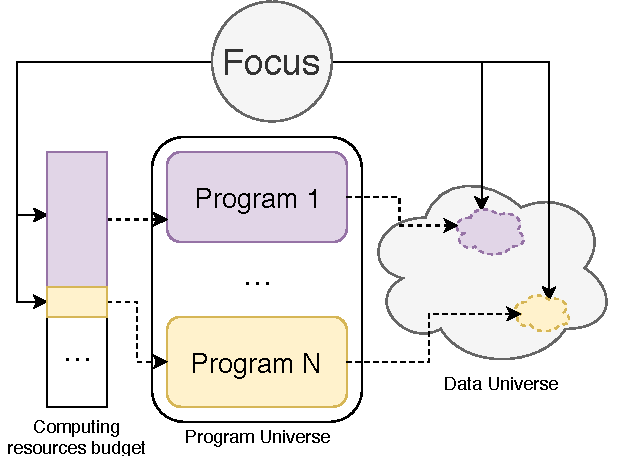
\includegraphics[width=0.7\linewidth]{./img/mind.pdf}\label{fig:mind}
    \caption{High level overview of the attention phenomenon. Attention is responsible for selecting programs to which computing resources should be applied and also data to be used by the programs.}
\end{figure}

\subsection{Attributes of Attention}
We now describe in more details each component of the attention phenomenon
as modeled in this work.

\subsubsection{Continuity}\label{sec:attrs-continuity}
The continuity of the process may be even \emph{hard} or \emph{soft}.
This division has been popular in Deep Learning research lately.

For \emph{hard} attention, the selection is \emph{discrete}:
the process performs selection of a subset of the targets.
One example of hard selection is the process of
choosing a specific subset of $k$ feature vectors (from $m \ge k$ options)
to be further processed.

For \emph{soft} attention, the selection is \emph{continuously} spread accross the
targets. It can be seen as of type of `weighting'' spread accross the targets.
Using the example above, the selection of feature vectors could be soft ---
in this case, instead of selecting a subset of vectors, every vector
could be given a weight $0 \le w \le 1$ for a subsequent convex combination.

\subsubsection{Subjects}\label{sec:attrs-subjects}
As mentioned before,
the subject of the focus (i.e.\ the target type) may be either \emph{data} or \emph{programs}.

Selection of \emph{data} regards selecting targets that are to be used as input
to other processes.
Data can be thought of as a vector of arbitrary dimensionality.
We can further classify this selection based on the \emph{semantic meaning}
of the selection:
\begin{itemize}
    \item \textbf{Location-based}: based on the location of the stimuli, such as the coordinates of a pixel.
    \item \textbf{Feature-based}: based on the features of a stimuli, such as color, orientation.
    \item \textbf{Object-based}: based on semantic elements of the stimuli, such as a specific toy in an image.
\end{itemize}
It is worth noting that, in the end, every data selection can be considered to be location-based.
After all, the targets of selection will always be discrete items of a vector (pixels of an image, for example).
This further semantic division is nonetheless useful.

An example of a process of selection of data
is the selection of a subregion of the input image to be processed
in an image classification task.
In this case, selection can be considered to be location-based.
If the selection chooses a discrete subset of the pixels, it can be
considered to be hard.
If, however, the selection takes place as producing a
heatmap mapping each pixel to a continuous value, the selection can be
considered to be soft.

\begin{figure}[H]
    \centering
    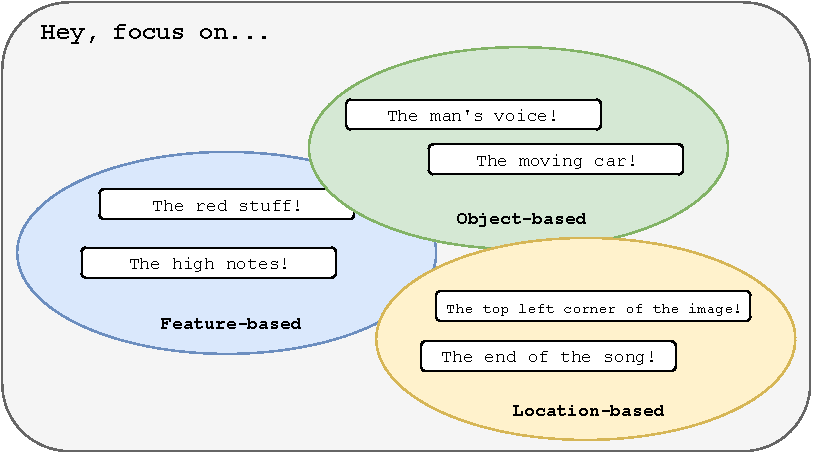
\includegraphics[width=0.8\linewidth]{./img/dataselsem.pdf}\label{fig:dataselsem}
    \caption{Examples of data selection semantic meanings.}
\end{figure}

\subsubsection{Flow}\label{sec:attrs-flow}
The \emph{flow} (or course) of \emph{selection along time} in a process
can be classified as \emph{ephemeral} or \emph{enduring}.

Ephemeral refers to selection of subjects in the context of a \emph{short time window}.
The evolution of selection along time is not important --- only the instantaneous selection is.
For example, in a task of visual control of a car,
an attention process to identify the abrupt appearance of moving obstacles
could be considered ephemeral since it does not take into account
much context and only happens during a short time window.

Enduring refers to the process of selection of objects over a \emph{long time window}.
The enduring focus can be further classified as:
\begin{itemize}
    \item \textbf{Oriented}: An arbitrary focus sequence so as to complete a certain task.
    \item \textbf{Sustained}: Focus restrained to a subset of the targets.
    \item \textbf{Divided}: Focus alternating among a subset of the targets.
\end{itemize}
Using the example of visual control of a car,
constantly focusing on the road would be considered \emph{sustained} selecttion.
Reading the signs of the road is an \emph{oriented} process since the focus must correctly follow the sequence of letters.
Alternatting focus among the mirrors, the speedometer and the road can be considered to be \emph{divided} selection.

\begin{figure}[H]
    \centering
    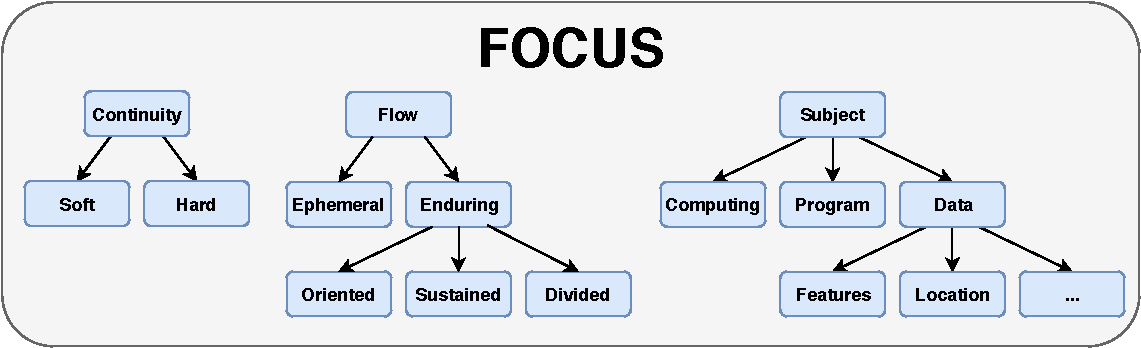
\includegraphics[width=1.0\linewidth]{./img/taxonomy.pdf}\label{fig:taxonomy}
    \caption{Attention attributes.}
\end{figure}

\section{Attentional Module}
We propose that the process of Attention --- as discussed in Section~\ref{sec:taxonomy}  --- can emerge by means of \emph{a series of components} --- which we call \emph{attentional modules}. These modules can alter data being processed and the execution flow of the algorithm and provide the functionalities of Attention.

\begin{figure}[H]
    \centering
    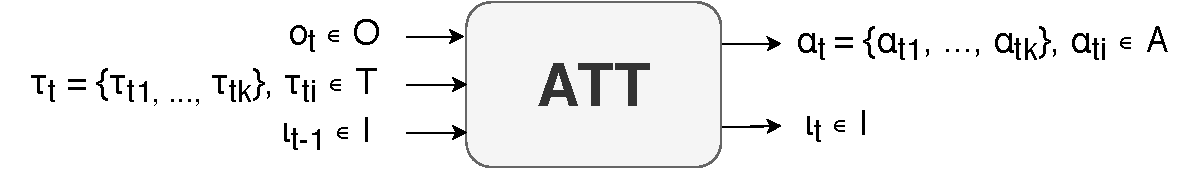
\includegraphics[width=0.9\linewidth]{./img/alt_att_block.pdf}\label{fig:attmodule}
    \caption{Attentional module.}
\end{figure}

Figure~\ref{fig:attmodule} illustrates the attentional module. At each time step $t$, the module receives as \emph{input}:
\begin{itemize}
    \item Current \emph{outer state} $o_t \in O$, where $O$ is the \emph{outer state set}.
    \item Group of \emph{focus targets} $\tau_t = \{\tau_{t1}, \ldots, \tau_{tk}\}, \tau_{ti} \in T$,
        where $T$ is the \emph{focus target set}.
    \item Past \emph{inner state} $\iota_{t-1} \in I$, where $I$ is the \emph{inner state set}.
\end{itemize}

The module produces as \emph{output} (as a function of both inputs):
\begin{itemize}
    \item Current \emph{inner state} $\iota_t \in I$.
    \item Current \emph{focus output} $\alpha_t = \{\alpha_{t1}, \ldots, \alpha_{tk}\}, \alpha_{ti} \in A$,
        where $A$ is the \emph{focus output set}.
\end{itemize}

The focus output is the main element of the module: it can be used to allocate \emph{finite resources} to a set of ``candidate targets'' by giving them an ``importance score'' which can be used in any arbitrary way in following steps.
Each element $\alpha_{tk}$ is respective to a target element $\tau_{tk}$.

\subsection{Modules and the attributes of Attention}
A system with Attention may contain more than one attentional modules --- even in a recursive manner.
Together, these modules always perform the function to provide selection capabilities
as discussed in Section~\ref{sec:taxonomy}.
We now provide some examples of how the attentional modules can act to provide such functionalities.

\subsubsection{Soft and Hard selection}
The different selection continuities (Section~\ref{sec:attrs-continuity})
can be obtained by means of attentional modules in the following manner:
\begin{itemize}
    \item \textbf{Soft selection}:
        $A = [0, 1]$, with $0 \le \sum_{i=1}^{k} \alpha_{ti} \le 1$
    \item \textbf{Hard selection}:
        $A = \{0, 1\}$, with $0 \le \sum_{i=1}^{k} \alpha_{ti} \le M$ and $0 \le M \le |\tau_t|$
\end{itemize}

\subsubsection{Subjects of selection}
Although the subjects selection (Section~\ref{sec:attrs-subjects})
differentiatie between programs and data, to the modules everything
can be treated simply as data. We provide some examples below.

\textbf{Selection of a single program}:
In this example, the system executes only one program at once and must
select the next task to be executed.
We can consider the target set $T$ to be the set of possible $N$ programs
and use hard attention: $A \in \{0, 1\}$, with $0 \le \sum_{i=1}^{N} \alpha_{ti} \le 1$.

\textbf{Program selection --- allocation of computing time}:
In this example, the system contains only one program $p$ to be executed but
must decide how much computation to ``spend'' (from the ``budget'' $B$) on the program at a certain timestep.
We can set the target set $T$ to be $\{p, nop\}$ (considering $nop$ to be doing nothing) and
use soft attention: $A \in [0, 1]$, with $\alpha_{t1} + \alpha_{t2} = 1$.
Thus, the amount of computation can be calculated as $\alpha_{t1}B$.

\textbf{Selection of data --- focusing on part of an image}:
In this example, the system must select a window of size $H\times W$ of the image to further perform classification.
The focus targets $\tau_t$ at time $t$ may represent the set of pixels $p_t$ of the current input image
with $N \ge H \times W$ pixels.
We can use hard attention and set the focus output set
$A \in \{0, 1\}$, with $\sum_{i=1}^{N} \alpha_{ti} = 1$,
so that $\alpha_{ti} = 1$ if and only if the window should be centered at pixel $p_{ti}$.

\textbf{Feature-based selection of data --- focusing more on certain colors}:
In this example, the system must give weights (summing to 1) to the channels R, G, B of the input image.
The focus targets $\tau_t$ at time $t$ may represent the respective channels: $\{R_{t}, G_{t}, B_{t}\}$
use soft attention: $A \in [0, 1]$, with $\alpha_{t1} + \alpha_{t2} + \alpha_{t3} = 1$.

Note that the semantic objects of data selection often cannot be directly modeled
as they refer to a high level and subjective context, but
such type of selection (and other higher level functionalities)
can nonetheless emerge by means of a combination of modules that ir right for the task.

\subsubsection{Selection flow type}
We provide below some examples of how the different selection flow types (Section~\ref{sec:attrs-subjects})
can emerge with modules.

\textbf{Ephemeral flow selection}:
Such type of selection takes place during a short
time window and state is usually not important.
Thus, we can simply model it by means of a module with the inner state at any time $t$ to be
null: $\iota_t = \emptyset$.

\textbf{Enduring flow selection}:
Selection flows which take place along a long time window usually require
information about the past, so the inner state must be non-empty: $\iota_t \ne \emptyset$.

\textbf{Sustained flow selection}:
Sustained flow can be achieved, for example, by using
one attentional module followed by another.
Suppose there are $M$ target elements to be selected and we want to restrict
our analysis to a subset of $N \le M$ elements.
The fist module selects such subset in a fixed manner for some amount of time:
$A \in \{0, 1\}$, with $\sum_{i=1}^{M} \alpha_{ti} = N$.
The target set of the next module is then the set of selected elements:
$\{\tau_{ti}: \alpha_{ti} = 1\}$.

\subsubsection{Example of an entire system}
Figure~\ref{fig:attsystem} shows the diagram of a possible system with attention.
The module \emph{TaskATT} uses hard attention to select a certain task $k$ to be executed for some time at time step $t$.
Among the computations of task $k$, there is the module \emph{DataATT}, which uses soft attention to allocate resources to a set of items.
It is worth noting that time is relative to each attentional module: \emph{TaskATT} has a temporal course over time steps $t$ that is different from that of \emph{DataATT}, which is over time steps $t'$.
Also, their sets of inputs and outputs may differ.
Together, these modules provide two types of focus:
\emph{hard}, \emph{enduring}/\emph{oriented} focus on \emph{programs} and
\emph{soft}, \emph{ephemeral} focus on data.

\begin{figure}[H]
    \centering
    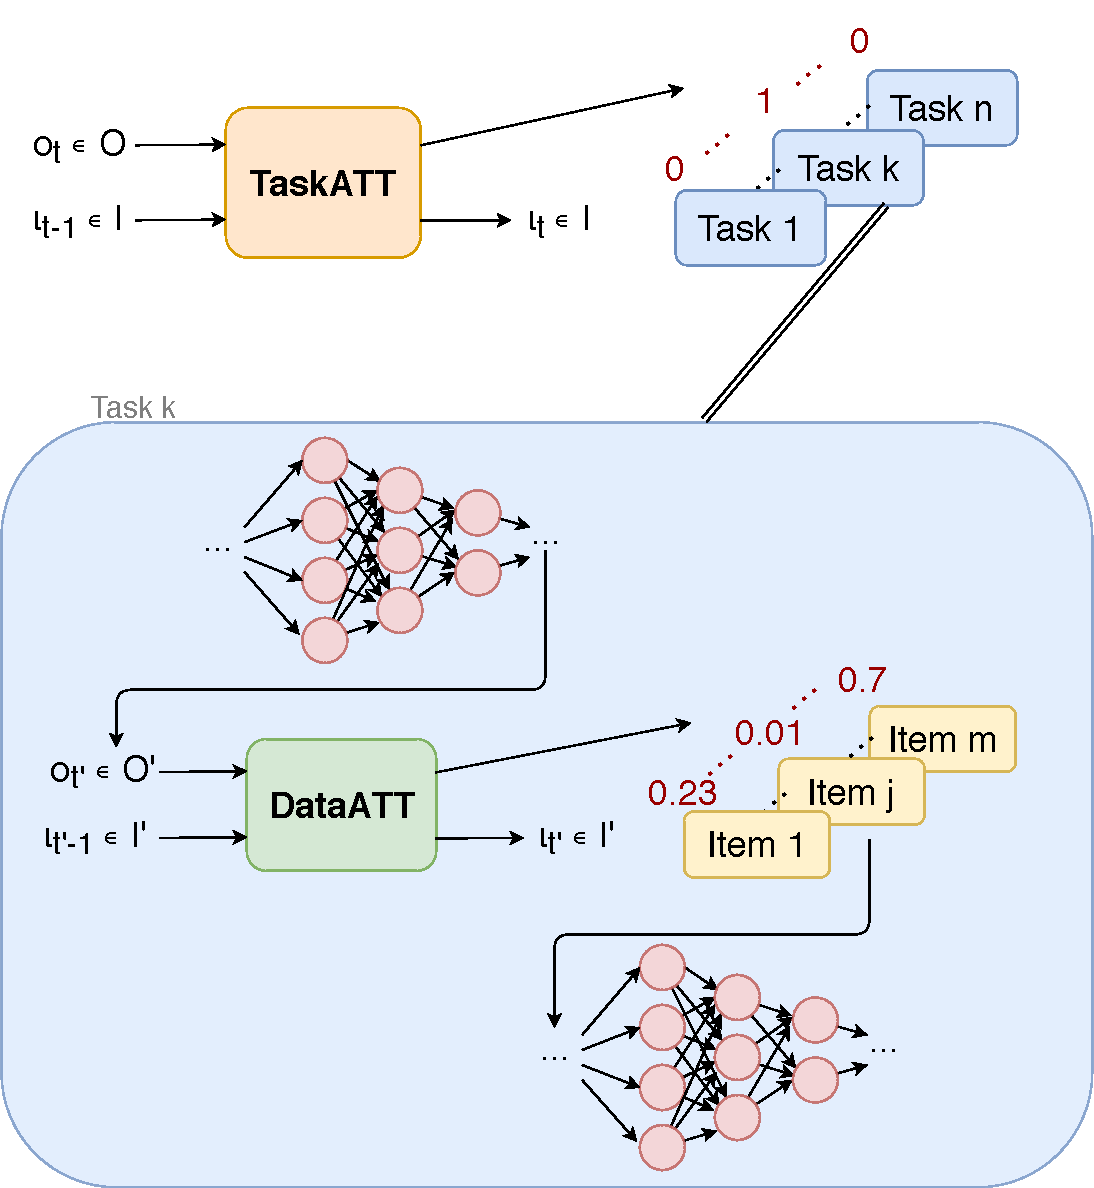
\includegraphics[width=0.8\linewidth]{./img/att_blocks_example.pdf}\label{fig:attsystem}
    \caption{Example of a system that uses attention.}
\end{figure}

\section{Validating the framework}
In this section, we investigate some recent works on attention and see how they fit in our framework.

\subsection{Image Caption Generation}
The work~\cite{ref:show-attend-tell} is among the first to propose using
attention to image caption generation: the encoding of the input image is
represented as a set of vectors --- each respective to a certain spatial region of the image ---
and the attentional component gives weights to each vector at each step in order to produce another
vector to be used in further computations.

\begin{figure}[H]
    \centering
    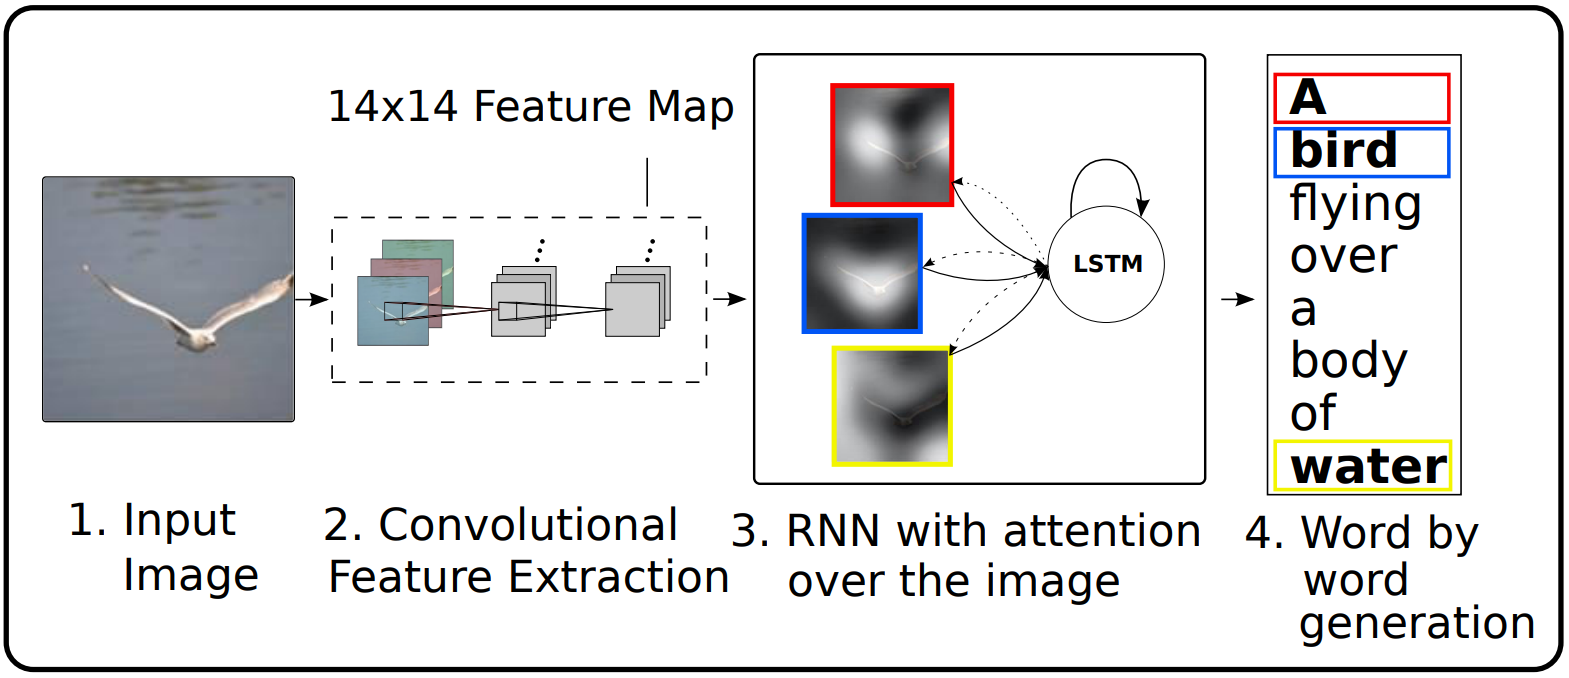
\includegraphics[width=0.8\linewidth]{./img/img_captioning.png}\label{fig:imgcaptioning}
    \caption{Diagram of natural language image description using Attention
    (from~\cite{ref:img-captioning}).}
\end{figure}

While there are many abstract processing substeps in the process, the \emph{end-to-end} effect is that of
a focus with \emph{soft} continuity, with \emph{orienting} flow, targetting \emph{data}
on a \emph{Location-based} manner. Figure~\ref{fig:imgcaptioning} illustrates the proposed model.

\begin{figure}[H]
    \centering
    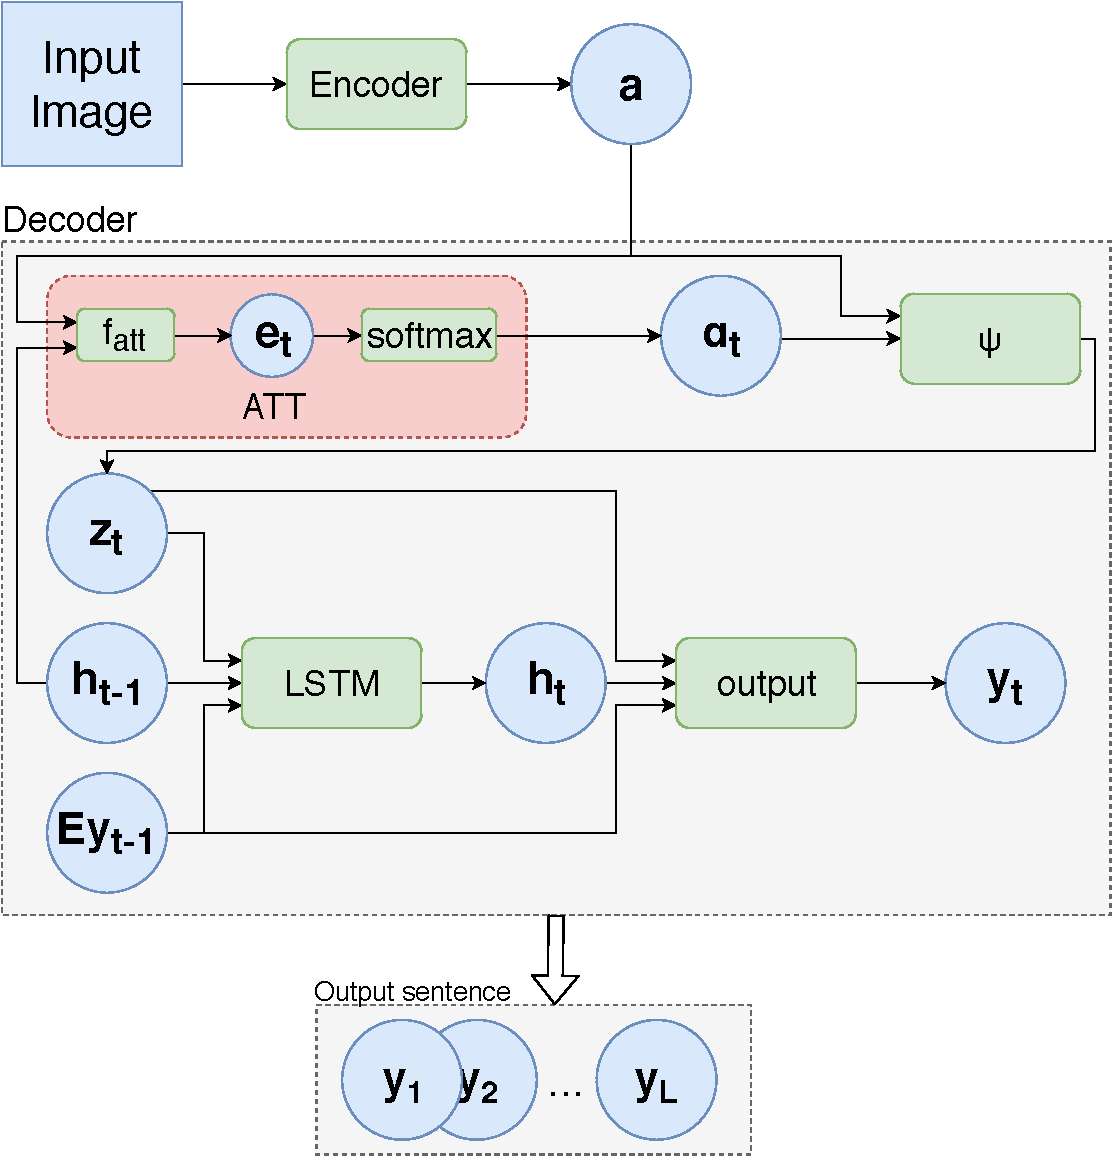
\includegraphics[width=0.8\linewidth]{./img/captioning.pdf}\label{fig:captioning}
    \caption{Model proposed for image captioning in~\cite{ref:show-attend-tell} with attentional module.}
\end{figure}

Figure~\ref{fig:captioning} illustrates the model proposed in the work.
The steps that calculate the attention to each encoding vector can be ``encapsulated'' as
an attentional module under our modeling:
$a$, the input image encoding, is the \emph{focus target input} $\tau_t$,
$h_{t-1}$, the hidden state of the model LSTM, is the \emph{outer state input} $o_t$
and $\alpha_t$, the weights given to each encoding vector, is the \emph{focus output}. In this case, $A = [0, 1]$.
Note that, in this case, the \emph{internal state} is empty.

\subsection{Adaptive Computation Time}
The work~\cite{ref:act} proposes an RNN that can perform a variable number of computation ``sub-steps'' for each time step $t'$.
The main idea is to calculate an amount $0 \le p_{t',t} \le 1$ to be ``spent'' for each computation sub-step $t$ up until the
moment the total spent reaches the ``budget'' of $1$ (in which moment the computation is halted).
The final value $y_{t'}$ is computed as an weighted average of the intermediate $y_{t',t}$ values and the weights are the values
$p_{t',t}$.

\begin{figure}[H]
    \centering
    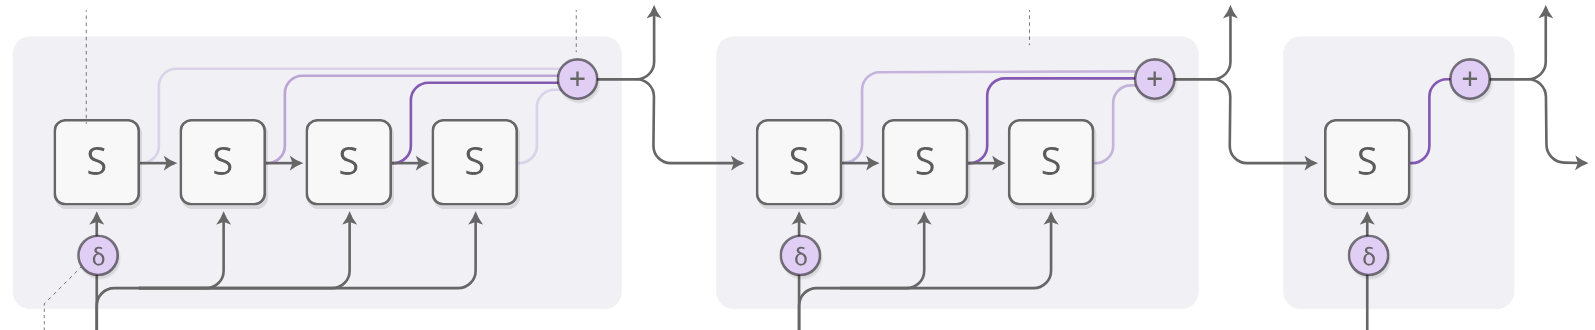
\includegraphics[width=0.8\linewidth]{./img/adaptive_comp.png}\label{fig:adct}
    \caption{Adaptive computation time process illustration.}
\end{figure}

The attention component provides two types of focus:
The selection of computing substeps at each step can be thought as a focus flow with \emph{soft} continuity,
\emph{oriented} signature and \emph{programs} (in this case, only one program and halting are options)
as selection target.
The computation of the result of each step uses \emph{soft} selection of \emph{ephemeral}
signature and \emph{data} as focus target.

\begin{figure}[H]
    \centering
    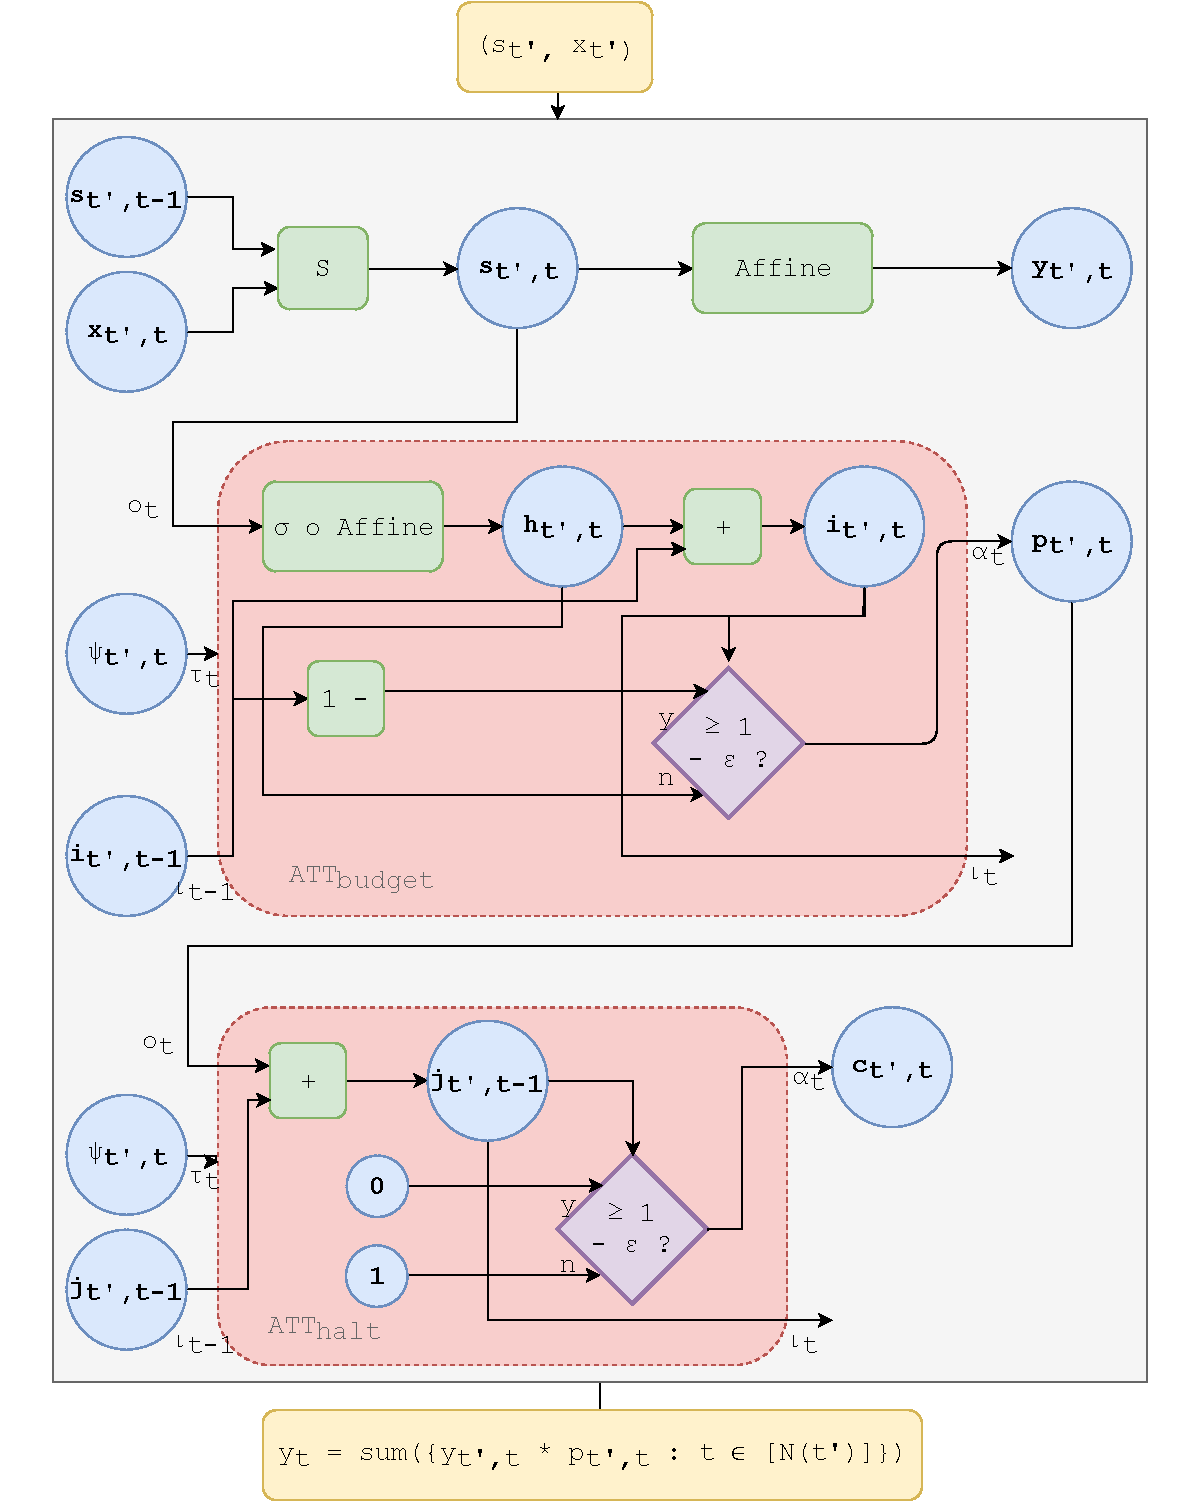
\includegraphics[width=0.75\linewidth]{./img/act.pdf}\label{fig:act}
    \caption{Model proposed for image captioning in~\cite{ref:act} with attentional module.}
\end{figure}

Figure~\ref{fig:act} illustrates the model proposed in the work.
The proposed model can be thought as having two attention modules:
\begin{itemize}
    \item \textbf{$ATT_{budget}$}, which computes the value $0 \le p_{t',t} \le 1$ to be spent at a given sub-step.
        In this analogy, $s_{t',t}$ --- the state of the RNN cell --- is the \emph{outer state} $o_t$;
        $\psi_t$ --- a dummy element representing the current computation sub-step --- is the \emph{target} $\tau_t$;
        and $i_{t',t}$ is the \emph{inner state}.
        The \emph{focus output} $p_{t',t}$, besides representing values to be consumed from the budget,
        can be thought of as an importance weight for the final output $y_t$, since the produced values are used to computed
        the weighted average.
    \item \textbf{$ATT_{halt}$}, which computes the value $c_{t',t} \in \{0, 1\}$, which is $1$ if the cell should continue
        further sub-steps and $0$ otherwise.
        In this analogy, $p_{t',t}$ is the \emph{outer state} $o_t$;
        $\psi_t$ --- a dummy element representing the current computation sub-step --- is the \emph{target} $\tau_t$;
        and $j_{t',t}$ is the \emph{inner state}.
\end{itemize}

\subsection{Recurrent Attention Model of Visual Attention}
The work~\cite{ref:ram} proposes a general recurrent model that uses visual attention at each step
by selecting a ``retina-like'' representation of a portion of the input image to carry out further computations.
At each time step $t$, the model uses the selected location $l_{t-1}$ to extract a retina-like representation
from input image.
An arbitrary action $a_t$ can be executed to possibly alter the environment.

\begin{figure}[H]
    \centering
    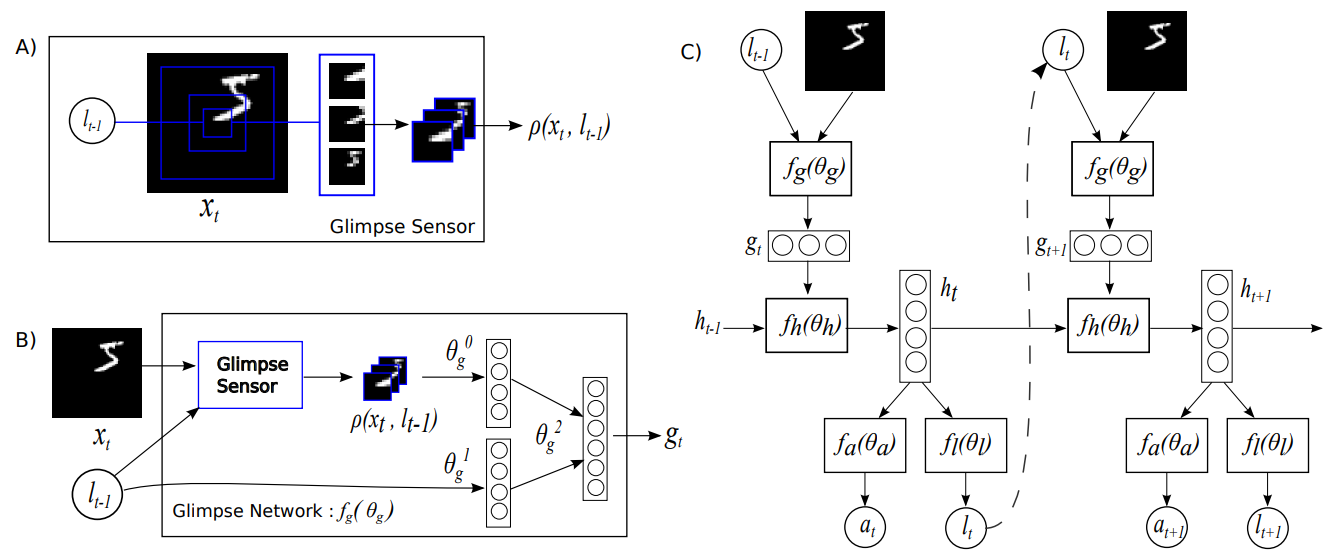
\includegraphics[width=1.0\linewidth]{./img/ram.png}
    \caption{General recurrent architecture proposed in~\cite{ref:ram}.}
\end{figure}

The attention component in the proposed model can be thought as providing
\emph{hard}, \emph{oriented} selection of \emph{data} in a \emph{location-based} manner.

\begin{figure}[H]
    \centering
    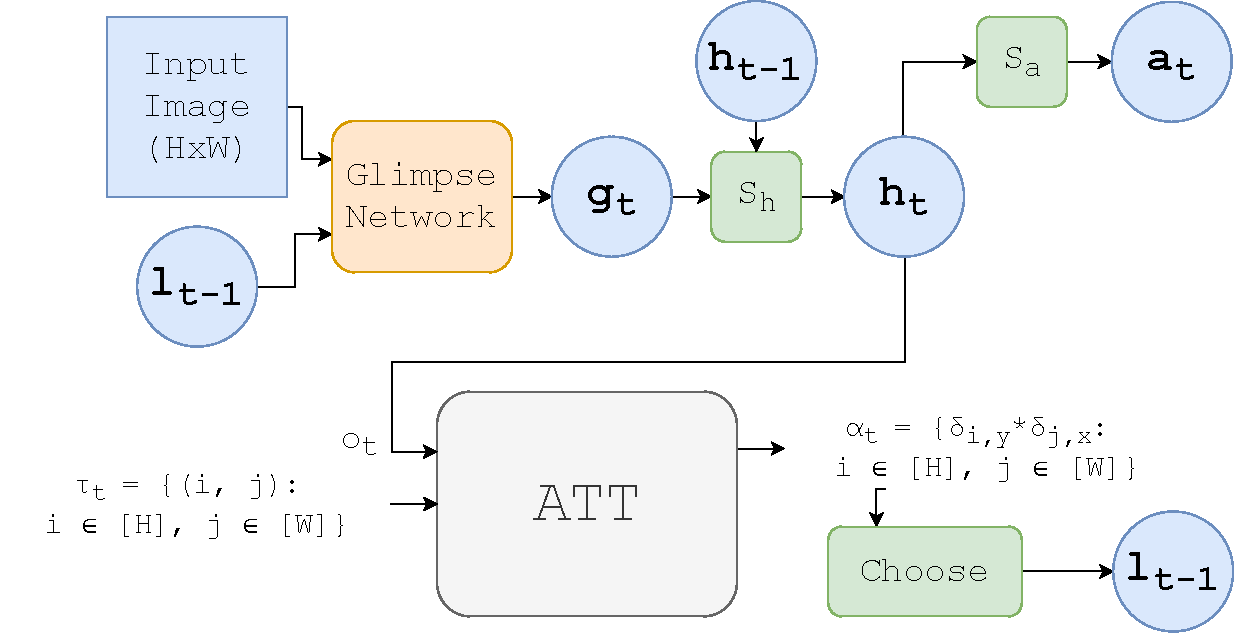
\includegraphics[width=0.7\linewidth]{./img/ram.pdf}\label{fig:ram}
    \caption{General recurrent architecture proposed in~\cite{ref:ram} with attentional module.}
\end{figure}

Figure~\ref{fig:ram} illustrates the model proposed in the work.
In this representation, the hidden state of the RNN $h_t$ is the \emph{outer state} input $o_t$;
The set of possible pixel coordinates $\{(i, j): i \in [H], j \in [W]\}$ (with $H, W$ as the height, width of the image)
is the \emph{focus targets} input $\tau_t$;
and the set $\{\delta_{i, y}\delta_{j, x}: i \in [H], j \in [W]\}$ is the \emph{focus output}.
Note that only the element $\delta_{i, y}\delta_{j,x}$ --- which is respective to the chosen pixel coordinates $(x, y)$
is equal to $1$.

Table~\ref{tab:tx} summarizes the taxonomy of the works cited above.
\begin{table}[H]
\centering
\caption{\small Taxonomy of cited works.}
    \begin{tabular}{|c|c|c|c|}
	\hline
     Work & Focus continuity & Focus flow & Focus subject\\
    \hline~\cite{ref:show-attend-tell} & Soft & Oriented & Data/Object-based\\
    \hline~\cite{ref:act} & Hard & Oriented & Program\\
    \hline~\cite{ref:act} & Soft & Ephemeral & Data\\
    \hline~\cite{ref:ram} & Hard & Oriented & Data/Location-based\\
    \hline
\end{tabular}\label{tab:tx}
\end{table}

\printbibliography\end{document}
